\documentclass{article}\usepackage[]{graphicx}\usepackage[]{color}
%% maxwidth is the original width if it is less than linewidth
%% otherwise use linewidth (to make sure the graphics do not exceed the margin)
\makeatletter
\def\maxwidth{ %
  \ifdim\Gin@nat@width>\linewidth
    \linewidth
  \else
    \Gin@nat@width
  \fi
}
\makeatother

\definecolor{fgcolor}{rgb}{0.345, 0.345, 0.345}
\newcommand{\hlnum}[1]{\textcolor[rgb]{0.686,0.059,0.569}{#1}}%
\newcommand{\hlstr}[1]{\textcolor[rgb]{0.192,0.494,0.8}{#1}}%
\newcommand{\hlcom}[1]{\textcolor[rgb]{0.678,0.584,0.686}{\textit{#1}}}%
\newcommand{\hlopt}[1]{\textcolor[rgb]{0,0,0}{#1}}%
\newcommand{\hlstd}[1]{\textcolor[rgb]{0.345,0.345,0.345}{#1}}%
\newcommand{\hlkwa}[1]{\textcolor[rgb]{0.161,0.373,0.58}{\textbf{#1}}}%
\newcommand{\hlkwb}[1]{\textcolor[rgb]{0.69,0.353,0.396}{#1}}%
\newcommand{\hlkwc}[1]{\textcolor[rgb]{0.333,0.667,0.333}{#1}}%
\newcommand{\hlkwd}[1]{\textcolor[rgb]{0.737,0.353,0.396}{\textbf{#1}}}%

\usepackage{framed}
\makeatletter
\newenvironment{kframe}{%
 \def\at@end@of@kframe{}%
 \ifinner\ifhmode%
  \def\at@end@of@kframe{\end{minipage}}%
  \begin{minipage}{\columnwidth}%
 \fi\fi%
 \def\FrameCommand##1{\hskip\@totalleftmargin \hskip-\fboxsep
 \colorbox{shadecolor}{##1}\hskip-\fboxsep
     % There is no \\@totalrightmargin, so:
     \hskip-\linewidth \hskip-\@totalleftmargin \hskip\columnwidth}%
 \MakeFramed {\advance\hsize-\width
   \@totalleftmargin\z@ \linewidth\hsize
   \@setminipage}}%
 {\par\unskip\endMakeFramed%
 \at@end@of@kframe}
\makeatother

\definecolor{shadecolor}{rgb}{.97, .97, .97}
\definecolor{messagecolor}{rgb}{0, 0, 0}
\definecolor{warningcolor}{rgb}{1, 0, 1}
\definecolor{errorcolor}{rgb}{1, 0, 0}
\newenvironment{knitrout}{}{} % an empty environment to be redefined in TeX

\usepackage{alltt}
\usepackage{amscd, amssymb, amsmath, verbatim, setspace}
\usepackage[left=1.0in, right=1.0in, top=1.0in, bottom=1.0in]{geometry}
\usepackage{mathrsfs}
\usepackage{listings}


\IfFileExists{upquote.sty}{\usepackage{upquote}}{}
\begin{document}
\begin{flushright}
Arif Ali\\
Math 640 Bayesian Statistics\\
May 11, 2016\\
\end{flushright}

\begin{center}
\LARGE\textbf{Final Exam}
  \end{center}
\section*{Exercise 1}
\subsection*{Part A}
\begin{equation}
\begin{split}
F(x)=\int_{k}^{x}\theta k^{\theta}*x^{-(\theta+1)}dx=\theta k^{\theta}\int_{k}^{x}x^{-(\theta+1)}dx=\theta k^{\theta}\big|_{k}^{x}-\frac{1}{\theta}x^{-\theta}dx=\theta k^{\theta}\left(-\frac{1}{\theta}x^{-\theta}+\frac{1}{\theta}k^{-\theta}\right)= \\
1-\left(\frac{k}{x}\right)^{\theta}
\end{split}
\end{equation} 


Let $u\sim unif(0,1)$

\begin{equation}
\begin{split}
u = F(x)\implies u = 1-\left(\frac{k}{x}\right)^{\theta}\implies (1-u) = \left(\frac{k}{x}\right)^{\theta}\implies(1-u)^{1/\theta} = \left(\frac{k}{x}\right) \implies x = \frac{k}{(1-u)^{1/\theta}}\\
\therefore F^{-1}(x) = \frac{k}{(1-x)^{1/\theta}}
\end{split}
\end{equation} 

Obtain a random sample, u, from $U\sim unif(0,1)$. Obtain x by computing $F^{-1}(x)$ and ensure that the values of $x\leq k$ will be evaluated to zero (this will only occur when u = 0).
\subsection*{Part B}
\begin{knitrout}
\definecolor{shadecolor}{rgb}{1, 1, 1}\color{fgcolor}\begin{kframe}
\begin{verbatim}
set.seed(1)
k=2
theta = 3
u = runif(1e6)
X = k/(1-u)^(1/theta)
X[u==0]=0
\end{verbatim}
\end{kframe}
\end{knitrout}
\subsection*{Part C}
\begin{knitrout}
\definecolor{shadecolor}{rgb}{1, 1, 1}\color{fgcolor}\begin{kframe}
\begin{verbatim}
hist(X[X<10], breaks = 50)
\end{verbatim}
\end{kframe}
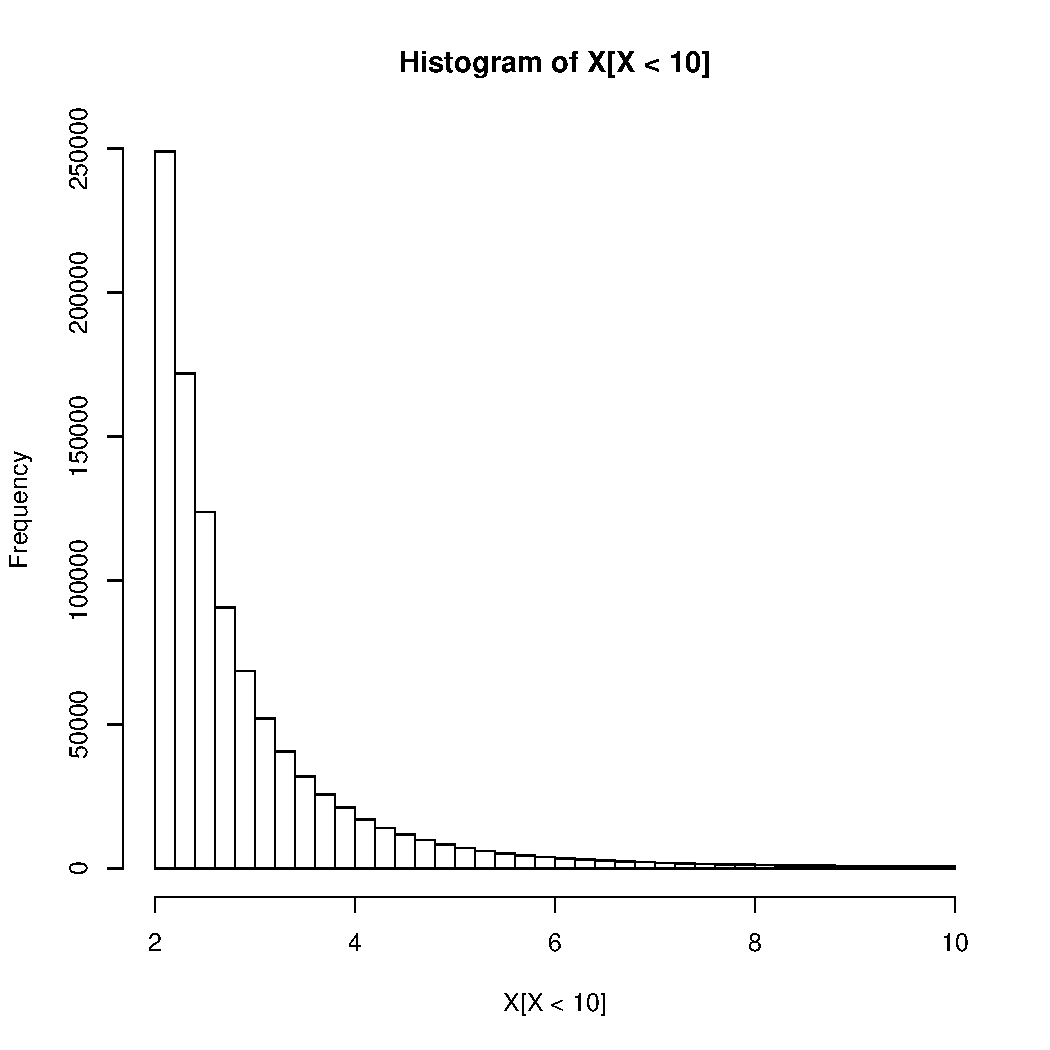
\includegraphics[width=0.50\linewidth]{figure/unnamed-chunk-3-1} 
\begin{kframe}\begin{verbatim}
x = seq(0,10, 0.01)
plot(x, 3*2^3/x^4, col = "red", type = "l")
\end{verbatim}
\end{kframe}
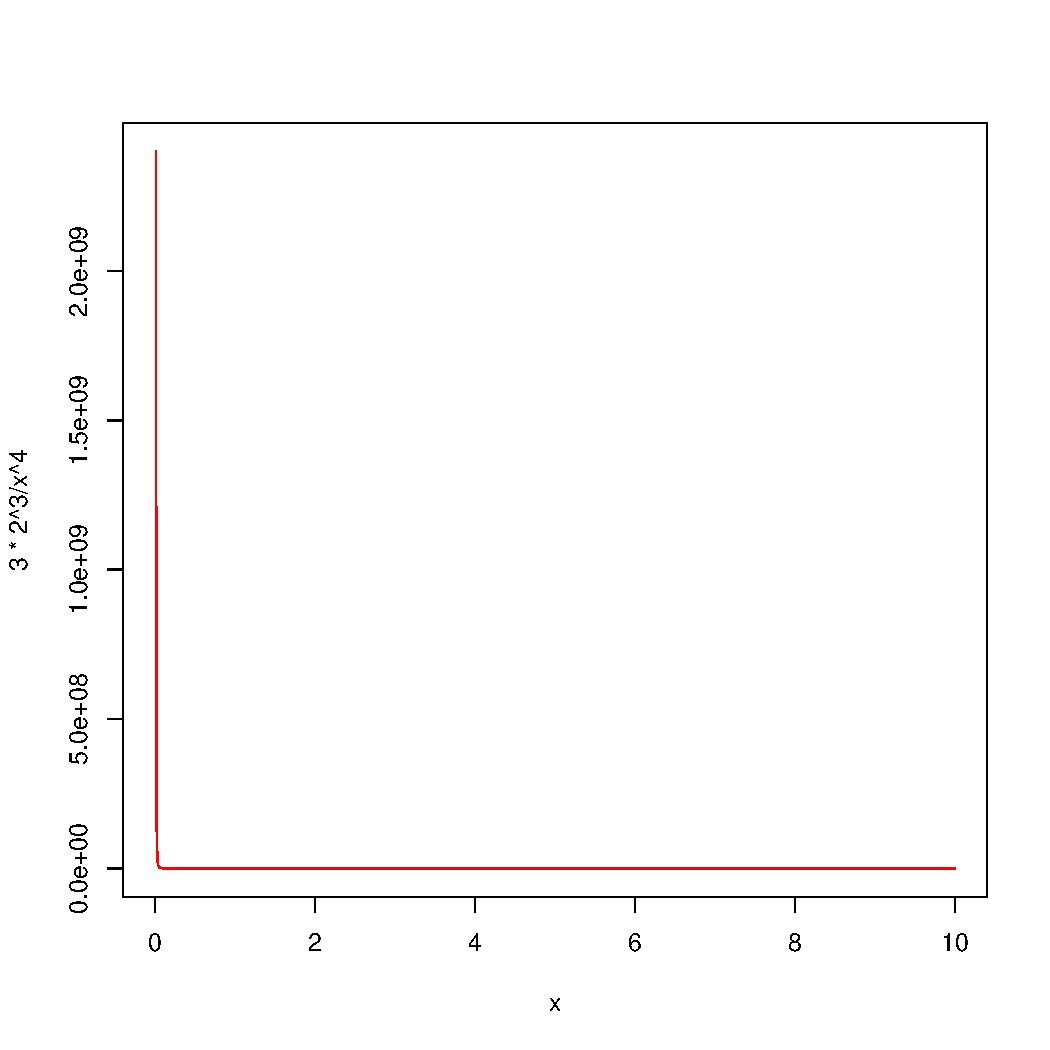
\includegraphics[width=0.50\linewidth]{figure/unnamed-chunk-3-2} 

\end{knitrout}
\subsection*{Part D}
$P(X<3)=F(x=3)=1-(\frac{2}{3})^{3})=0.7037037$
\begin{knitrout}
\definecolor{shadecolor}{rgb}{1, 1, 1}\color{fgcolor}\begin{kframe}
\begin{verbatim}
mean(X<3)
## [1] 0.703963
\end{verbatim}
\end{kframe}
\end{knitrout}
\newpage
\section*{Exercise 2}

\end{document}
